\documentclass[border=3pt]{standalone}
\usepackage[T1]{fontenc}
\usepackage{helvet}
\renewcommand{\familydefault}{\sfdefault}
\usepackage{tikz}
\usetikzlibrary{arrows.meta,positioning,fit,backgrounds,shapes.geometric,calc}
\definecolor{ink}{HTML}{1F3A56}
\definecolor{core}{HTML}{DCE7F2}
\definecolor{know}{HTML}{DDEFE8}
\definecolor{game}{HTML}{F6E8D6}
\definecolor{model}{HTML}{EAE3F3}
\definecolor{plain}{HTML}{F3F4F6}
\definecolor{bad}{HTML}{B3402E}
\tikzset{
 every node/.style={font=\fontsize{8.5}{10.2}\selectfont,align=center,text=ink,execute at begin node={\hyphenpenalty=10000\exhyphenpenalty=10000}},
 box/.style={draw=ink,fill=white,rounded corners=1.5pt,minimum height=8.5mm,inner sep=3pt,line width=.5pt},
 corebox/.style={box,fill=core},
 knowbox/.style={box,fill=know},
 gamebox/.style={box,fill=game},
 modelbox/.style={box,fill=model},
 plainbox/.style={box,fill=plain},
 planned/.style={dashed},
 flow/.style={-{Stealth[length=2mm]},draw=ink,line width=.6pt},
 dflow/.style={flow,dashed},
 badflow/.style={flow,draw=bad,dashed},
 band/.style={draw=ink!55,rounded corners=3pt,inner sep=6pt,line width=.45pt},
 title/.style={font=\bfseries\fontsize{8.5}{10.2}\selectfont},
 lab/.style={font=\fontsize{7.5}{9}\selectfont,fill=white,inner sep=1pt},
 decision/.style={diamond,draw=ink,fill=core,aspect=2.1,inner sep=0.5pt,line width=.5pt}
}

\begin{document}
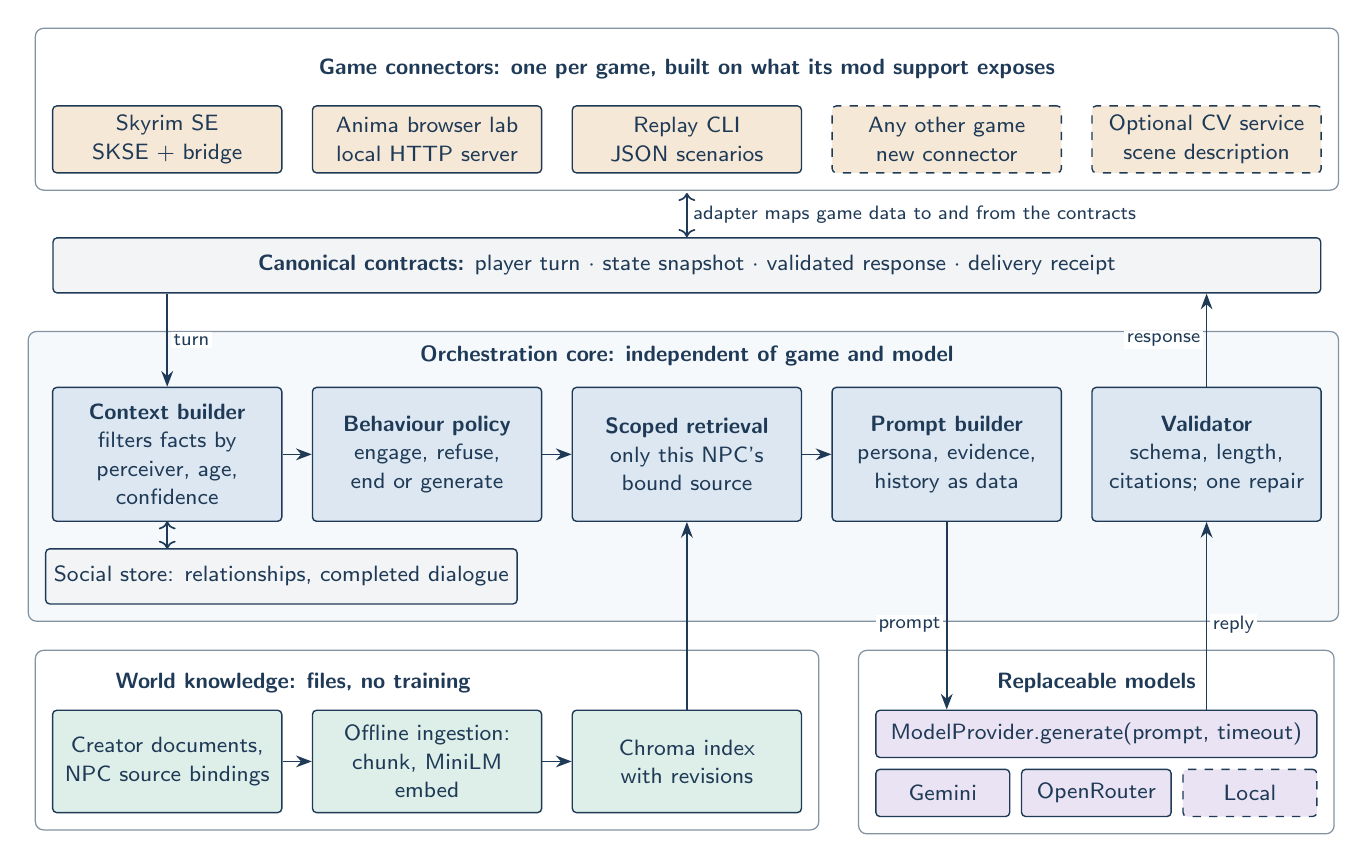
\begin{tikzpicture}[x=1mm,y=1mm]
\def\bw{29mm}
% Column centres: 16, 49, 82, 115, 148
% Connectors
\node[title] at (82,63) {Game connectors: one per game, built on what its mod support exposes};
\node[gamebox,minimum width=\bw,text width=27mm] (sky) at (16,54) {Skyrim SE\\SKSE + bridge};
\node[gamebox,minimum width=\bw,text width=27mm] (lab) at (49,54) {Anima browser lab\\local HTTP server};
\node[gamebox,minimum width=\bw,text width=27mm] (rep) at (82,54) {Replay CLI\\JSON scenarios};
\node[gamebox,planned,minimum width=\bw,text width=27mm] (new) at (115,54) {Any other game\\new connector};
\node[gamebox,planned,minimum width=\bw,text width=27mm] (cv) at (148,54) {Optional CV service\\scene description};
\begin{scope}[on background layer]
\node[band,fit={(sky)(cv)(82,66)}] (games) {};
\end{scope}
% Contract
\node[plainbox,minimum width=161mm,minimum height=7mm] (contract) at (82,38)
 {\textbf{Canonical contracts:} player turn $\cdot$ state snapshot $\cdot$ validated response $\cdot$ delivery receipt};
\draw[flow,<->] (82,47.2) -- node[lab,right=1pt] {adapter maps game data to and from the contracts} (contract.north);
% Core
\node[title] at (82,26.5) {Orchestration core: independent of game and model};
\node[corebox,minimum width=\bw,text width=27mm,minimum height=17mm] (ctx) at (16,14) {\textbf{Context builder}\\filters facts by perceiver, age, confidence};
\node[corebox,minimum width=\bw,text width=27mm,minimum height=17mm] (pol) at (49,14) {\textbf{Behaviour policy}\\engage, refuse, end or generate};
\node[corebox,minimum width=\bw,text width=27mm,minimum height=17mm] (ret) at (82,14) {\textbf{Scoped retrieval}\\only this NPC's bound source};
\node[corebox,minimum width=\bw,text width=27mm,minimum height=17mm] (pro) at (115,14) {\textbf{Prompt builder}\\persona, evidence, history as data};
\node[corebox,minimum width=\bw,text width=27mm,minimum height=17mm] (val) at (148,14) {\textbf{Validator}\\schema, length, citations; one repair};
\node[plainbox,minimum width=58mm,minimum height=7mm] (state) at (30.5,-1.5) {Social store: relationships, completed dialogue};
\draw[flow] (ctx) -- (pol);
\draw[flow] (pol) -- (ret);
\draw[flow] (ret) -- (pro);
\draw[flow,<->] (16,5.5) -- (16,2);
\draw[flow] (contract.south -| ctx.north) -- node[lab,right=1pt] {turn} (ctx.north);
\draw[flow] (val.north) -- node[lab,left=1pt] {response} (contract.south -| val.north);
\begin{scope}[on background layer]
\node[band,fill=core!25,fit={(ctx)(val)(state)(82,27.5)}] (coreband) {};
\end{scope}
% Knowledge
\node[title] at (32,-15) {World knowledge: files, no training};
\node[knowbox,minimum width=\bw,text width=27mm,minimum height=13mm] (docs) at (16,-25) {Creator documents, NPC source bindings};
\node[knowbox,minimum width=\bw,text width=27mm,minimum height=13mm] (idx) at (49,-25) {Offline ingestion: chunk, MiniLM embed};
\node[knowbox,minimum width=\bw,text width=27mm,minimum height=13mm] (db) at (82,-25) {Chroma index\\with revisions};
\draw[flow] (docs) -- (idx);
\draw[flow] (idx) -- (db);
\draw[flow] (db.north) -- (ret.south);
\begin{scope}[on background layer]
\node[band,fit={(docs)(db)(49,-13)}] (kband) {};
\end{scope}
% Models
\node[title] at (134,-15) {Replaceable models};
\node[modelbox,minimum width=56mm,minimum height=6mm] (mp) at (134,-21.5) {ModelProvider.generate(prompt, timeout)};
\node[modelbox,minimum width=17mm,minimum height=6mm] (gem) at (114.5,-29) {Gemini};
\node[modelbox,minimum width=19mm,minimum height=6mm] (orr) at (134,-29) {OpenRouter};
\node[modelbox,planned,minimum width=17mm,minimum height=6mm] (loc) at (153.5,-29) {Local};
\begin{scope}[on background layer]
\node[band,fit={(mp)(gem)(loc)(134,-13)}] (mband) {};
\end{scope}
\draw[flow] (pro.south) -- node[lab,left=1pt,pos=.55] {prompt} (mp.north -| pro.south);
\draw[flow] (mp.north -| val.south) -- node[lab,right=1pt,pos=.45] {reply} (val.south);
\end{tikzpicture}
\end{document}
